\subsection{三角形的内角和}\label{subsec:czjh1-3-3}

在小学,我们曾经把一个三角形纸板的三个角拼在一起,发现它们组成一个平角(图 \ref{fig:czjh1-3-10})。
这表明,三角形三个内角的和等于 $180^\circ$。就是

\begin{dingli}[三角形内角和定理]
    三角形三个内角的和等于 $180^\circ$。
\end{dingli}

\begin{figure}[htbp]
    \centering
    \begin{minipage}[b]{7cm}
        \centering
        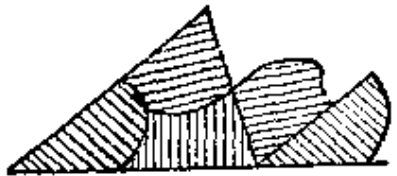
\includegraphics[width=5cm]{../pic/czjh1-ch3-10.png}
        \caption{}\label{fig:czjh1-3-10}
    \end{minipage}
    \qquad
    \begin{minipage}[b]{7cm}
        \centering
        \begin{tikzpicture}
    \tkzDefPoints{0/0/B, 3.5/0/C, 2.8/2/A}
    \tkzDefPointOnLine[pos=1.5](B,C)  \tkzGetPoint{D}
    \tkzDefLine[parallel=through C, normed](B,A) \tkzGetPoint{e}
    \tkzDefPointOnLine[pos=1.5](C,e)  \tkzGetPoint{E}

    \tkzDrawPolygon(A,B,C)
    \tkzDrawSegments[dashed](C,D  C,E)
    \tkzMarkAngles[size=0.3](E,C,A)
    \tkzMarkAngles[size=0.5](D,C,E)
    \tkzLabelAngle[pos=0.5](E,C,A){$1$}
    \tkzLabelAngle[pos=0.7](D,C,E){$2$}
    \tkzLabelPoints[above](A,E)
    \tkzLabelPoints[below](B,C,D)
\end{tikzpicture}


        \caption{}\label{fig:czjh1-3-11}
    \end{minipage}
\end{figure}

下面我们来证明这个定理。

已知:$\triangle ABC$(图 \ref{fig:czjh1-3-11})。

求证:$\angle A + \angle B + \angle C = 180^\circ$。

分析:实验是把三个内角拼在一起组成一个平角,这启发我们,要证明这个命题,
可先以 $CA$ 为一边,在 $\triangle ABC$ 的外部作 $\angle ACE = \angle A$,
再延长 $BC$, 然后只要能证明 $\angle ECD = \angle B$ 就可以了。

\zhengming 作 $BC$ 的延长线 $CD$, 在 $\triangle ABC$ 的外部,
以 $CA$ 为一边, $CE$ 为另一边作 $\angle 1 = \angle A$ (图 \ref{fig:czjh1-3-11})。 于是

\hspace*{2em} $CD \pingxing BA$(内错角相等,两直线平行)。

$\therefore$ \quad $\angle B = \angle 2$ (两直线平行,同位角相等)。

又 $\because$ $\angle 1 + \angle 2 + \angle ACB = 180^\circ$(平角的定义),

$\therefore$ \quad $\angle A + \angle B + \angle ACB = 180^\circ$ (等量代换)。

为了证明的需要,在原来图形上添画的线叫做\zhongdian{辅助线}。
在平面几何里,辅助线通常画成虚线。

从上面的证明过程可以知道, $\angle ACD = \angle A + \angle B$, 由此得到:

\begin{tuilun}[推论1]
    三角形的一个外角等于和它不相邻的两个内角的和。
\end{tuilun}

\begin{tuilun}[推论2]
    三角形的一个外角大于任何一个和它不相邻的内角。
\end{tuilun}


\begin{wrapfigure}[8]{r}{6cm}
    \centering
    \begin{tikzpicture}
    \tkzDefPoints{0/0/B, 3.5/0/C, 2.8/2/A}
    \tkzDefPointOnLine[pos=1.3](A,B)  \tkzGetPoint{D}
    \tkzDefPointOnLine[pos=1.3](B,C)  \tkzGetPoint{E}
    \tkzDefPointOnLine[pos=1.3](C,A)  \tkzGetPoint{F}

    \tkzDrawPolygon(A,B,C)
    \tkzDrawSegments(B,D  C,E  A,F)
    \tkzMarkAngles[size=0.4](B,A,C  C,B,A  A,C,B)
    \tkzLabelAngle[pos=0.6](B,A,C){$1$}
    \tkzLabelAngle[pos=0.6](C,B,A){$2$}
    \tkzLabelAngle[pos=0.6](A,C,B){$3$}
    \tkzLabelPoints[right](A)
    \tkzLabelPoints[left](F)
    \tkzLabelPoints[above left](B)
    \tkzLabelPoints[below](C,D,E)
\end{tikzpicture}


    \caption{}\label{fig:czjh1-3-12}
\end{wrapfigure}

\liti[0] 已知:$\angle BAF$、$\angle CBD$、$\angle ACE$ 是 $\triangle ABC$ 的三个外角(图 \ref{fig:czjh1-3-12})。

求证: $\angle BAF + \angle CBD + \angle ACE = 360^\circ$。

\zhengming 如图,$\because$ \quad $\angle BAF = \angle 2 + \angle 3$,
$\angle CBD = \angle 1 + \angle 3$, $\angle ACE = \angle 1 + \angle 2$
(三角形的一个外角等于和它不相邻的两个内角的和),

$\therefore$ \quad $\angle BAF + \angle CBD + \angle ACE = 2(\angle 1 + \angle 2 + \angle 3)$ (等式性质)。

$\because$ \quad $\angle 1 + \angle 2 + \angle 3 = 180^\circ$ (三角形内角和定理),

$\therefore$ \quad $\angle BAF + \angle CBD + \angle ACE = 2 \times 180^\circ = 360^\circ$ (等量代换)。

由内角和定理我们知道,三角形的每一个内角都不大于 $180^\circ$,
所以一个三角形的三个内角可能都是锐角,也可能有一个是直角或钝角,
因此,三角形可以按角进行分类。

\begin{figure}[htbp]
    \centering
    \begin{minipage}[b]{4.5cm}
        \centering
        \begin{tikzpicture}
    \tkzDefPoints{0/0/B, 3.5/0/C, 1.1/2/A}

    \tkzDrawPolygon(A,B,C)
    \tkzLabelPoints[above](A)
    \tkzLabelPoints[below](B,C)
\end{tikzpicture}


        \caption*{甲}
    \end{minipage}
    \qquad
    \begin{minipage}[b]{4cm}
        \centering
        \begin{tikzpicture}
    \tkzDefPoints{0/0/B, 2/0/C, 2/3/A}

    \tkzDrawPolygon(A,B,C)
    \tkzMarkRightAngle(A,C,B)
    \tkzLabelPoints[above](A)
    \tkzLabelPoints[below](B,C)
\end{tikzpicture}


        \caption*{乙}
    \end{minipage}
    \begin{minipage}[b]{4cm}
        \centering
        \begin{tikzpicture}
    \tkzDefPoints{0/0/B, 1.5/0/C, 2.5/3/A}

    \tkzDrawPolygon(A,B,C)
    \tkzLabelPoints[above](A)
    \tkzLabelPoints[below](B,C)
\end{tikzpicture}


        \caption*{丙}
    \end{minipage}
    \caption{}\label{fig:czjh1-3-13}
\end{figure}


三个角都是锐角的三角形叫做\zhongdian{锐角三角形}(图 \ref{fig:czjh1-3-13} 甲)。
有一个角是直角的三角形叫做\zhongdian{直角三角形}(图 \ref{fig:czjh1-3-13} 乙)。
有一个角是钝角的三角形叫做\zhongdian{钝角三角形}(图 \ref{fig:czjh1-3-13} 丙)。
锐角三角形和钝角三角形合称\zhongdian{斜三角形}。

$$
    \text{三角形} \smash[t]{\left\{ \begin{aligned}
        &\text{直角三角形} \\[1.5em]
        & \text{斜三角形} \smash{\left\{ \begin{aligned}
            &\text{锐角三角形} \\
            &\text{钝角三角形}
        \end{aligned} \right.}
    \end{aligned} \right.}
$$ \vspace*{.5em}

在直角三角形中,夹直角的两边叫做\zhongdian{直角边}, 直角的对边叫做\zhongdian{斜边}。
两条直角边相等的直角三角形叫做\zhongdian{等腰直角三角形}。


\begin{lianxi}

\xiaoti{(口答) 一个三角形中,能否有两个内角是钝角或直角?为什么?}

\xiaoti{画一个 $\triangle ABC$, 再画出它的所有外角。 如果 $\angle BAC = 50^\circ$, $\angle ABC = 60^\circ$,
    那么 $\angle ACB$ 等于多少度? 与 $\angle ACB$ 相邻的一个外角等于多少度?为什么?
}

\xiaoti{已知:如图,$P$ 是 $\triangle ABC$ 内一点, 延长 $BP$ 交 $AC$ 于 $D$。\\
    求证:(1)$\angle 1 > \angle 2$; (2)$\angle 2 > \angle A$;(3)$\angle 1 > \angle A$。
}

\begin{figure}[htbp]
    \centering
    \begin{minipage}[b]{7cm}
        \centering
        \begin{tikzpicture}
    \tkzDefPoints{0/0/B, 3.5/0/C, 2.4/2.5/A}
    \tkzDefPointOnLine[pos=0.5](A,C)  \tkzGetPoint{D}
    \tkzDefPointOnLine[pos=0.7](B,D)  \tkzGetPoint{P}

    \tkzDrawPolygon(A,B,C)
    \tkzDrawSegments(B,D  C,P)
    \tkzMarkAngles[size=0.3](B,P,C  B,D,C)
    \tkzLabelAngle[pos=0.5](B,P,C){$1$}
    \tkzLabelAngle[pos=0.5](B,D,C){$2$}
    \tkzLabelPoints[above](A,P)
    \tkzLabelPoints[below](B,C)
    \tkzLabelPoints[right](D)
\end{tikzpicture}


        \caption*{(第 3 题)}
    \end{minipage}
    \qquad
    \begin{minipage}[b]{7cm}
        \centering
        \begin{tikzpicture}
    \tkzDefPoints{0/0/A, 3.5/0/C}
    \tkzDefTriangle[school](A,C)  \tkzGetPoint{B}
    \tkzPermute(A,B,C) % 交换 B、C 坐标
    \tkzDefLine[altitude](A,C,B)  \tkzGetPoint{D}

    \tkzDrawPolygon(A,B,C)
    \tkzDrawSegments(C,D)
    \tkzMarkRightAngles(A,C,B  C,D,A)
    \tkzMarkAngles[size=0.5](A,C,D)
    \tkzMarkAngles[size=0.6](D,C,B)
    \tkzLabelAngle[pos=0.7](A,C,D){$1$}
    \tkzLabelAngle[pos=0.8](D,C,B){$2$}
    \tkzLabelPoints[above](C)
    \tkzLabelPoints[below](A,B,D)
\end{tikzpicture}


        \caption*{(第 4 题)}
    \end{minipage}
\end{figure}

\xiaoti{(口答〕如图, 已知 $\angle ACB = 90^\circ$, $CD \perp AB$, 垂足是 $D$。}
\begin{xiaoxiaotis}

    \xxt{图中有几个直角三角形? 是哪几个? 说出它们的直角边和斜边。}

    \xxt{$\angle 1 + \angle 2$ 等于多少度? $\angle B + \angle 2$ 等于多少度?为什么?
        $\angle 1$ 和 $\angle B$ 是不是相等?为什么?
    }

\end{xiaoxiaotis}

\end{lianxi}


